\section{Цель работы}
Изучение закономерностей колебательного движения тела в однородном поле силы тяжести; исследование процессов превращения энергии в консервативных системах; определение момента инерции физического маятника.

\section{Приборы и принадлежности}
\begin{wrapfigure}[13]{r}{0.25\textwidth}
    \centering
    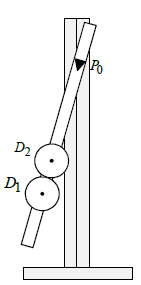
\includegraphics{маятник.png}
    \caption{}
    \label{fig:pendulum}
\end{wrapfigure}
Физический маятник; секундомер; масштабная линейка, чертежный треугольник.

Конструкция оборотного маятника представлена на рис. \ref*{fig:pendulum}. На стержне 1 закреплены два диска – D1 и D2. Маятник может быть подвешен на кронштейне к легкой
призме, трение в которой пренебрежимо мало.

\section{Исследуемые закономерности}

Физический маятник - это тело с распределенной массой или система тел, ось вращения которого расположена выше центра масс маятника. Относительно этой оси маятник колеблется с периодом
\begin{equation}\label{eq:Period}
    T_0=2 \pi \sqrt{\frac{I}{m g x_c}}=2 \pi \sqrt{\frac{l_0}{g}}
\end{equation}
где для составного маятника $m=\sum m_i$ - масса маятника, $x_c=\frac{1}{m} \sum m_i x_{c i}-$ положение его центра масс относительно оси вращения, $m_i$ и $x_{c i}-$ масса $i-$ го тела и положение его центра масс относительно оси вращения, $I=\sum I_i-$ полный момент инерции маятника, $I_i=I_{0 i}+m_i x_{c i}^2-$ момент инерции і-го тела, рассчитанный относительно оси вращения по теореме Штейнера, $I_{0 i}-$ момент инерции этого тела относительно его центра масс. Длина математического маятника, период которого совпадает с периодом колебаний данного физического маятника называется приведенной длиной физического маятника. Ее можно найти как $l_0=I / m x_c=g T_0^2 / 4 \pi^2$. Ее можно определить экспериментально, если найти новую ось $O^{\prime}$, называемую осью качания, относительно которой маятник колеблется с тем же периодом $T_0$, что и относительно оси вращения $O$. Расстояние между осями вращения и качания $O O^{\prime}=l_0$ и будет приведенной длиной физического маятника.
Полный момент инерции маятника может быть представлен в виде:
\begin{equation}\label{eq:fullMomentOfInertion}
    I=I_0+m \overline{x_c^2}
\end{equation}
где $I_0=\sum I_{0 i}, \overline{x_c^2}=\frac{1}{m} \sum m_i x_{c i}^2-$ средний квадрат положений центров масс системы тел, составляющих маятник.

Если период колебаний маятника определен экспериментально, то из
\eqref{eq:Period} можно найти момент инерции маятника:
\begin{equation}\label{eq:momentOfInertion}
    I=m g x_{\mathrm{c}} T_0^2 / 4 \pi^2 .
\end{equation}
\subsection{Сохранение энергии гармонических колебаний.}
Поскольку физический маятник, качающийся под действием силы тяжести, является консервативной системой, можно проанализировать процесс перехода потенциальной энергии маятника в кинетическую и обратно.

Потенциальная энергия при достижении амплитудного значения угла отклонения маятника равна:
\begin{equation}\label{eq:potentionEnergy}
    W_{\mathrm{pm}}=m g h_{\mathrm{c}}=m g x_{\mathrm{c}}\left(1-\cos \varphi_{\mathrm{m}}\right)=2 m g x_{\mathrm{c}} \sin ^2 \frac{\varphi_{\mathrm{m}}}{2} \approx \frac{1}{2} m g x_{\mathrm{c}} \varphi_{\mathrm{m}}^2
\end{equation}

где $h_c$ - высота поднятия центра масс маятника при его максимальном отклонении от положения равновесия, $x_{\mathrm{c}}-$ положение центра масс маятника относительно его точки подвеса, $\varphi_{\mathrm{m}}-$ максимальный угол отклонения маятника от положения равновесия.

При малых углах отклонения маятника (до $20^{\circ}$ ) максимальная потенциальная энергия равна:
\begin{equation}\label{eq:maxPotentionEnergy}
    W_{\mathrm{pm}} \approx \frac{1}{2} m g x_{\mathrm{c}} \varphi_{\mathrm{m}}^2 .
\end{equation}
Максимальная кинетическая энергия физического маятника
\begin{equation}\label{eq:maxKeneticEnergy}
    W_{\mathrm{km}}=\frac{I \omega_{\mathrm{m}}^2}{2}=\frac{m g x_{\mathrm{c}} T_0^2 \omega_{\mathrm{m}}^2}{8 \pi^2},
\end{equation}
где момент инерции маятника выражен по формуле \eqref{eq:momentOfInertion} через период его колебаний. Из закона сохранения полной механической энергии
\begin{equation}\label{eq:conservationOfEnergy}
    W=W_k+W_p=W_{\mathrm{km}}=W_{\mathrm{pm}}=\text { const }
\end{equation}
можно найти максимальную угловую скорость маятника при прохождении им положения равновесия $\omega_{\mathrm{m}}=2 \pi \varphi_{\mathrm{m}} / T_0$.

\newpage
